\runningheader{SAT Mathematics}{Drill Set 14}{Page \thepage\ of \numpages}

\begingradingrange{sat-drill-14}
\subsection*{SAT Drill 14}


\question[1]
Consider the equation:
\[
  4|12-2 x|+12|6-x|=140
\]
What is the positive solution to the given equation?
\begin{solution}
13
\end{solution}

\question[1]
\begin{center}
  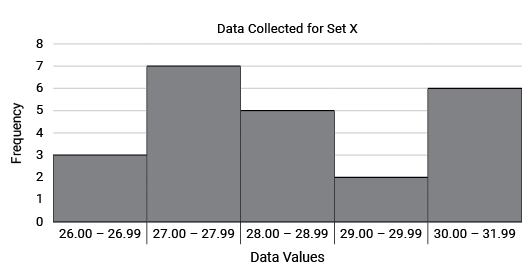
\includegraphics[width=0.60\linewidth]{images/cus48}
\end{center}
The histogram shows the data collected from set $X$. Data set $Y$ takes all the values from set $X$ and subtracts 17.5 to every value. Which of the following correctly compares the median and the range between set $X$ and set $Y$?
\begin{choices}
  \choice The median for set $X$ is greater than the median for set $Y$ and the range for set $X$ is greater than the range of set $Y$.
  \CorrectChoice The median for set $X$ is greater than the median for set $Y$ and the range for set $X$ is equal to the range of set $Y$.
  \choice The median for set $X$ is equal to the median for set $Y$ and the range for set $X$ is greater than the range of set $Y$.
  \choice The median for set $X$ is equal to the median for set $Y$ and the range for set $X$ is equal to the range of set $Y$.
\end{choices}

\question[1]
Function $g$ is defined by the equation $g(x)=8\left(\frac{1}{4}\right)^x$. If $h(x)=g(x+2)$, which of the following is the equation for $h(x)$?
\begin{choices}
  \CorrectChoice $h(x)=\frac{1}{2}\left(\frac{1}{4}\right)^x$
  \choice $h(x)=4\left(\frac{1}{4}\right)^x$
  \choice $h(x)=8\left(\frac{1}{4}\right)^x+2$
  \choice $h(x)=16\left(\frac{1}{2}\right)^x$
\end{choices}

\question[1]
The linear function $f(x)$ is defined such that $f(2)=13.5$ and $f(14)=22.5$. If $f(x+1)=18.75$, what is the value of $x$?
\begin{solution}
8
\end{solution}


\question[1]
Consider the equation:
\[
  0.5(1.5 x-0.75)=3\left(-\frac{x}{6}+\frac{1}{12}\right)
\]
What is the solution to the given equation?
\begin{solution}
$\frac{1}{2}$
\end{solution}


\question[1]
Consider the equation:
\[
  x^2-12 x+7=0
\]
One solution to the given equation can be written as $j-\sqrt{k}$, where $j$ and $k$ are constants. What is the value of $jk$?
\begin{solution}
174
\end{solution}

\question[1]
\begin{center}
  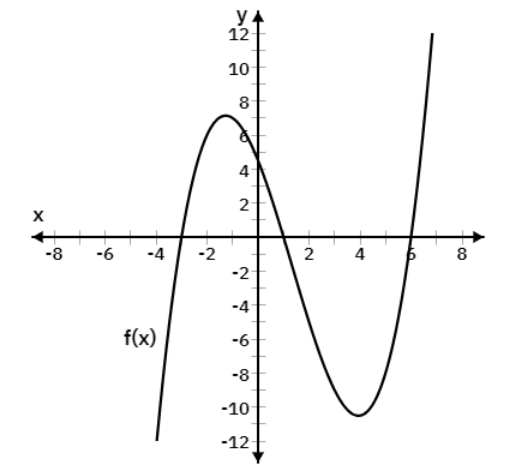
\includegraphics[width=0.40\linewidth]{images/cus49}
\end{center}
The graph of $y=f(x)$ is graphed on the $xy$-plane. The equation of $f(x)$ is represented by $f(x)=a(x+m)(x+n)(x+o)$, where $a, m, n$, and $o$ are constants. If the graph of $f(x)$ is moved one unit to the left, which of the following is true?
\statementbox{
  \begin{enumerate}[label=(\Roman*)]
    \item The value of $a$ decreases by 1
    \item The product of $m, n$, and $o$ is 0
    \item The $y$-intercept of the translated graph is at the origin
  \end{enumerate}
}
\begin{choices}
  \choice I only
  \choice I, II, and III
  \choice II only
  \choice II and III
\end{choices}

\question[1]
\begin{table}[h!]
\centering
\renewcommand{\arraystretch}{1.3}
\setlength{\tabcolsep}{16pt}
\begin{tabular}{|c|c|}
\hline
\rowcolor[HTML]{E0E0E0}
$x$ & $f(x)$ \\
\hline
-5 & -90 \\
\hline
-3 & 0 \\
\hline
0 & 0 \\
\hline
2 & -20 \\
\hline
4 & 0 \\
\hline
5 & 40 \\
\hline
\end{tabular}
\end{table}
The table above shows several values of the function $f$ graphed on the $xy$-coordinate plane. The equation of $f$ is defined by $f(x)=(x+a)(x+b)(x+c)$, where $a, b$, and $c$ are constants. Which of the following is true?
\statementbox{
  \begin{enumerate}[label=(\Roman*)]
    \item $a+b+c<0$
    \item $f(-2)<0$
    \item $f(-6)<f(6)$
  \end{enumerate}
}
\begin{choices}
  \choice I only
  \CorrectChoice I and III
  \choice I, II and III
  \choice III only
\end{choices}

  
\question[1]
Consider the function:
\[
  f(t)=155(1.14)^{\frac{4}{3} t}
\]
In the given function, the growth in revenue at a certain company is modeled, where $t$ represents years. According to the model, how many months does it take for the revenue to increase by $14\%$?
\begin{solution}
9
\end{solution}

\question[1]
\begin{center}
  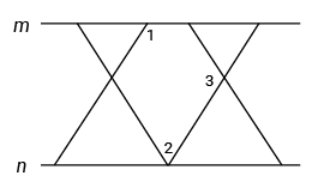
\includegraphics[width=0.40\linewidth]{images/cus50}
\end{center}
In the image shown, line $m$ is parallel to line $n$, all four triangles formed by the intersecting lines are isosceles triangles, and the two smaller triangles are congruent. If the measure of angle 3 is $104^{\circ}$, what is the sum of angle 1 and angle 2, in degrees?
\begin{choices}
  \choice 128
  \choice 204
  \choice 208
  \choice 256
\end{choices}



\question[1]
Let $t$ represent the number of tulips and $r$ represent the number of roses in a bouquet. Each tulip costs $\$3.50$ and each rose costs $\$5.25$. Flora wants to buy a bouquet for at most $\$50$ and have at least three times as many tulips as roses in the bouquet. Which system of inequalities best represents this scenario?
\begin{choices}
  \choice $\begin{aligned} & 3.50 t+5.25 r \leq 50 \\ & t \leq 3 r \end{aligned}$
  \choice $\begin{aligned} & 3.50 t+5.25 r \leq 50 \\ & 3 t \leq r \end{aligned}$
  \CorrectChoice $\begin{aligned} & 3.50 t+5.25 r \leq 50 \\ & t \geq 3 r \end{aligned}$
  \choice $\begin{aligned} & 3.50 t+5.25 r \leq 50 \\ & 3 t \geq r \end{aligned}$
\end{choices}

\question[1]
A quadratic equation with a leading coefficient of 1 intersects the $x$-axis at the points $(a, 0)$ and $(b, 0)$. What is the value of the $y$-coordinate of the vertex?
\begin{choices}
  \choice $-\frac{1}{4}(b-3 a)(b-a)$
  \CorrectChoice $-\frac{1}{4}(a-b)^2$
  \choice $\frac{1}{4}(a-b)^2$
  \choice $\frac{1}{4}(b-3 a)(b-a)$
\end{choices}


\question[1]
Two similar cylinders, Cylinder $A$ and Cylinder $B$, have volumes, in cubic meters, of $100 \pi$ and $800 \pi$ respectively. If the radius of Cylinder $A$ is equal to 2 meters, what is the total surface area of Cylinder $B$ in square meters? (Surface area of a cylinder $=2 \pi r(r+h)$)
\begin{choices}
  \choice $216 \pi$
  \choice $232 \pi$
  \CorrectChoice $432 \pi$
  \choice $864 \pi$
\end{choices}
  
\question[1]
The function $f$ is defined by the equation:
\[
  f(x) = |8 - 5x|
\]
For what value of $k$ does $f(k) = 6k + 3$?
\begin{solution}
$\frac{5}{11}$
\end{solution}

\question[1]
For groups of 28 or more people, an arcade charges $\$9$ per person for the first 28 people and $\$15$ for each additional person. How many total people were in attendance if the group paid $\$447$ to go to the arcade?
\begin{solution}
41
\end{solution}



\question[1]
The equation
\[
  3 x^2+18 x+3 y^2-6 y-15=0
\]
gives the graph of a circle in the $xy$-plane. If the circle is inscribed in a square, what is the area of the square?
\begin{solution}
60
\end{solution}



\question[1]
The function $f$ is defined by the given equation:
\[
  f(x)=5(0.92)^{3 x}
\]
The equation can be rewritten as $f(x)=5\left(1-\frac{p}{100}\right)^x$, where $p$ is a constant. Which of the following is closest to the value of $p$?
\begin{choices}
  \choice $8$
  \choice $12$
  \CorrectChoice $22$
  \choice $24$
\end{choices}



\question[1]
Consider the system of equations:
\[
  \begin{gathered}
  y=3 x^2-5 x-12 \\
  40 x-4 y=a
  \end{gathered}
\]
In the given system of equations, $a$ is a positive constant. The system has exactly one distinct real solution. What is the value of $a$?
\begin{solution}
123
\end{solution}

\question[1]
If the expression
\[
\frac{8-i}{3-2 i}
\]
is rewritten in the form $a+b i$, where $a$ and $b$ are real numbers, what is the value of $a$? (Note: $i=\sqrt{-1}$)
\begin{solution}
2
\end{solution}



\question[1]
In the $xy$-plane, the point $(p, r)$ lies on the line with equation $y = x + b$,
where $b$ is a constant. The point with coordinates $(2p, 5r)$ lies on the line
with equation $y = 2x + b$. If $p \neq 0$, what is the value of $\frac{r}{p}$?
\begin{choices}
  \choice $\frac{2}{5}$
  \CorrectChoice $\frac{3}{4}$
  \choice $\frac{4}{3}$
  \choice $\frac{5}{2}$
\end{choices}

\question[1]
For a polynomial $p(x)$, the value of $p(3)$ is $-2$. Which of the following must be true about $p(x)$?
\begin{choices}
  \choice $x-5$ is a factor of $p(x)$.
  \choice $x-2$ is a factor of $p(x)$.
  \choice $x+2$ is a factor of $p(x)$.
  \CorrectChoice The remainder when $p(x)$ is divided by $x-3$ is $-2$.
\end{choices}

\endgradingrange{sat-drill-14}
